%!TEX program = xelatex
\documentclass[12pt, a4paper]{article}

\usepackage[dvipsnames]{xcolor}

\usepackage{fancyhdr}
\usepackage{extramarks}
\usepackage{amsmath}
\usepackage{amsthm}
\usepackage{amsfonts}
\usepackage{tikz}
\usepackage[plain]{algorithm}
\usepackage{algpseudocode}

\usepackage{ctex}
\usepackage{indentfirst}
\usepackage{wrapfig}
\CTEXoptions[today=old]
\usetikzlibrary{automata,positioning,shapes.geometric,arrows.meta,patterns,calc}
\numberwithin{equation}{section}

%
% Basic Document Settings
%

\topmargin=-0.25in
\evensidemargin=0in
\oddsidemargin=0in
\textwidth=6.5in
\textheight=9.2in
\headsep=0.25in

\linespread{1.1}

\pagestyle{fancy}
\lhead{\hmwkAuthorName}
\chead{\hmwkClass : \hmwkTitle}
\rhead{\firstxmark}
\lfoot{\lastxmark}
\cfoot{\thepage}

\renewcommand\headrulewidth{0.4pt}
\renewcommand\footrulewidth{0.4pt}

\setlength{\parindent}{2em}  % 2em代表首行缩进两个字符

%
% Create Problem Sections
%

\newcommand{\enterProblemHeader}[1]{
    \nobreak\extramarks{}{Problem \arabic{#1} continued on next page\ldots}\nobreak{}
    \nobreak\extramarks{Problem \arabic{#1} (continued)}{Problem \arabic{#1} continued on next page\ldots}\nobreak{}
}

\newcommand{\exitProblemHeader}[1]{
    \nobreak\extramarks{Problem \arabic{#1} (continued)}{Problem \arabic{#1} continued on next page\ldots}\nobreak{}
    \stepcounter{#1}
    \nobreak\extramarks{Problem \arabic{#1}}{}\nobreak{}
}

% \setcounter{secnumdepth}{0}
\newcounter{partCounter}
\newcounter{homeworkProblemCounter}
\setcounter{homeworkProblemCounter}{0}
% \nobreak\extramarks{Problem \arabic{homeworkProblemCounter}}{}\nobreak{}

%
% Homework Problem Environment
%
% This environment takes an optional argument. When given, it will adjust the
% problem counter. This is useful for when the problems given for your
% assignment aren't sequential. See the last 3 problems of this template for an
% example.
%
\newenvironment{homeworkProblem}[1][-1]{
    \ifnum#1>0
        \setcounter{homeworkProblemCounter}{#1}
    \fi
    \section{Problem \arabic{homeworkProblemCounter}}
    \setcounter{partCounter}{1}
    \enterProblemHeader{homeworkProblemCounter}
}{
    \exitProblemHeader{homeworkProblemCounter}
}

%
% Homework Details
%   - Title
%   - Due date
%   - Class
%   - Section/Time
%   - Instructor
%   - Author
%

\newcommand{\hmwkTitle}{The Kinematics of Mass Points}
\newcommand{\hmwkDueDate}{\today}
\newcommand{\hmwkClass}{University Physics}
\newcommand{\hmwkClassTime}{}
\newcommand{\myUniversiy}{Wuhan University}
\newcommand{\hmwkAuthorName}{\textbf{Lai Wei}}

%
% Title Page
%

\title{
    \vspace{2in}
    \textmd{\textbf{\hmwkClass:\ \hmwkTitle}}\\
    \normalsize\vspace{0.1in}\small{Date: \hmwkDueDate}\\
    \vspace{0.1in}\large{\textit{\myUniversiy}}
    \vspace{3in}
}

\author{\hmwkAuthorName}
\date{}

\renewcommand{\part}[1]{\textbf{\large Part \Alph{partCounter}}\stepcounter{partCounter}\\}

%
% Various Helper Commands
%

% Useful for algorithms
\newcommand{\alg}[1]{\textsc{\bfseries \footnotesize #1}}

% % For derivatives
% \newcommand{\deriv}[1]{\frac{\mathrm{d}}{\mathrm{d}x} (#1)}

% For partial derivatives
\newcommand{\pderiv}[2]{\frac{\partial}{\partial #1} (#2)}

% Integral dx
\newcommand{\dx}{\mathrm{d}x}

% Alias for the Solution section header
\newcommand{\solution}{\textbf{\large Solution}}

% Probability commands: Expectation, Variance, Covariance, Bias
\newcommand{\E}{\mathrm{E}}
\newcommand{\Var}{\mathrm{Var}}
\newcommand{\Cov}{\mathrm{Cov}}
\newcommand{\Bias}{\mathrm{Bias}}

% 我的newcommand
\newcommand{\degree}{^{\circ}}
\newcommand{\arrow}{-{Stealth[length=4mm,width=2mm]}}
\newcommand{\rmd}{\mathrm{d}}
\newcommand{\deriv}[2]{\frac{\rmd #1}{\rmd #2}}
\renewcommand{\parallel}{\mathrel{/\mskip-2.5mu/}}

\begin{document}

\maketitle

\pagebreak

% 设置页码格式是罗马数字
\pagenumbering{roman}

% 生成目录
\tableofcontents

\pagebreak

% 设置页码格式是阿拉伯数字
\pagenumbering{arabic}

\pagebreak

\section{质点力学}

\subsection{参考系、质点}

\subsubsection{参考系}

    为描述物体运动而选的标准物。

\subsubsection{参考系}

    物体能否视为质点视具体情况而定。

\subsubsection{坐标系}

    定量描述物体运动。坐标系的原点一般固定在参照系上。

    \begin{enumerate}
        \item 直角坐标系\(\left(x,y,z\right)\)
        \item 球坐标系\(\left(r,\theta,\varphi\right)\):二维极坐标
        \item 柱坐标系\(\left(\rho,\varphi,z\right)\)
        \item 自然坐标系\(s\)
    \end{enumerate}

\subsection{位置矢量、运动方程、路程、位移}

\subsubsection{位置矢量}

    \begin{wrapfigure}{r}{4cm}
        \centering
        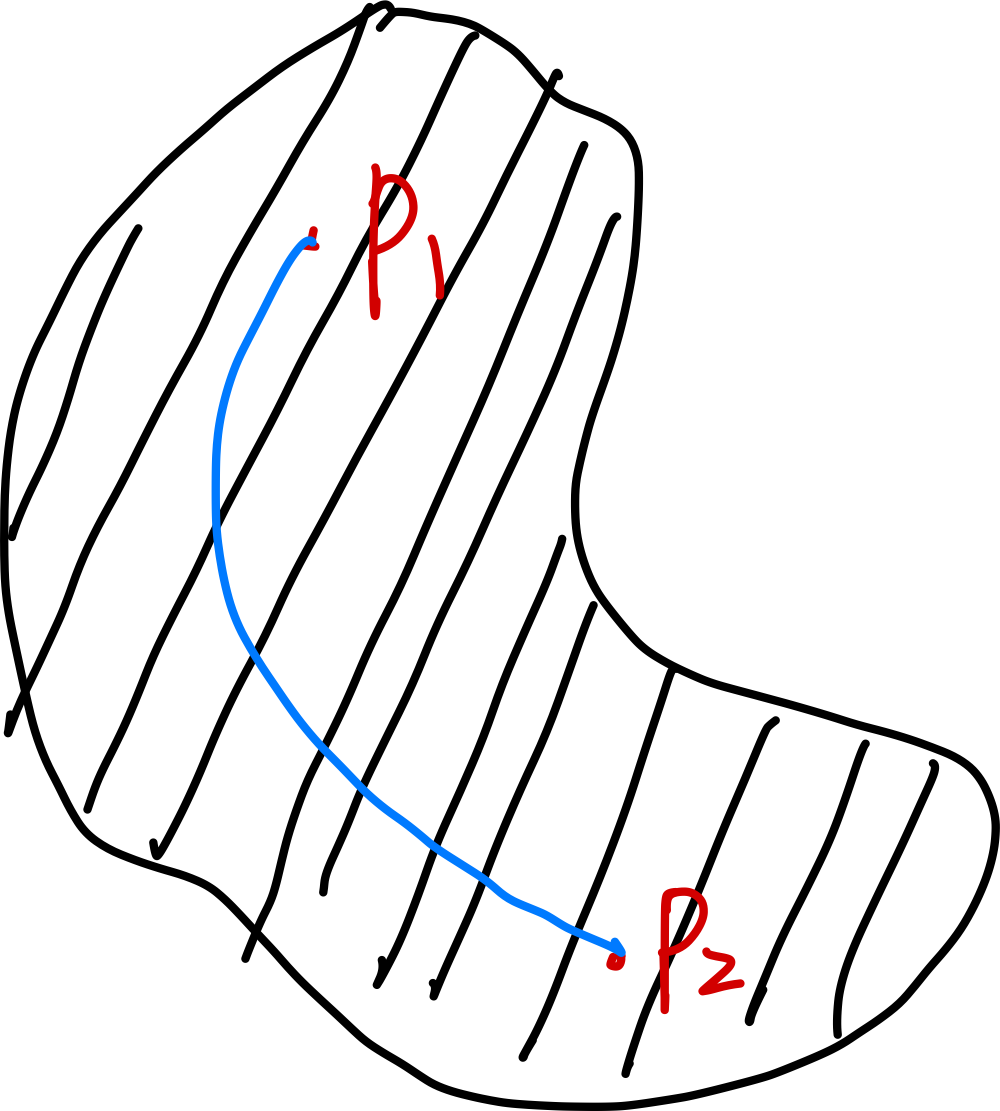
\includegraphics[scale=0.08]{"Chapter 01 images/pic1.png"}
        % \caption{}
        \label{pic1}
    \end{wrapfigure}

    \begin{align}
        \overrightarrow{r} &= x\overrightarrow{i} + y\overrightarrow{j} + z\overrightarrow{k} \\
        r &= \left|\overrightarrow{r}\right| = \sqrt{x^2 + y^2 + z^2}
    \end{align}

    \(\overrightarrow{r}\)的方向可以用一组方向角,即\(\overrightarrow{r}\)与\(x\)轴、
    \(y\)轴、\(z\)轴之间的夹角\(\left(\alpha, \beta, \gamma\right)\)来表示。
    \(\cos \alpha = \frac{x}{r}\)、\(\cos \beta = \frac{y}{r}\)、\(\cos \gamma = \frac{z}{r}\),
    有\(\cos \alpha ^2 + \cos \beta ^2 + \cos \gamma ^2 = 1\)。

\subsubsection{运动方程(直角坐标系下)}
    
    \begin{wrapfigure}{r}{4cm}
        \centering
        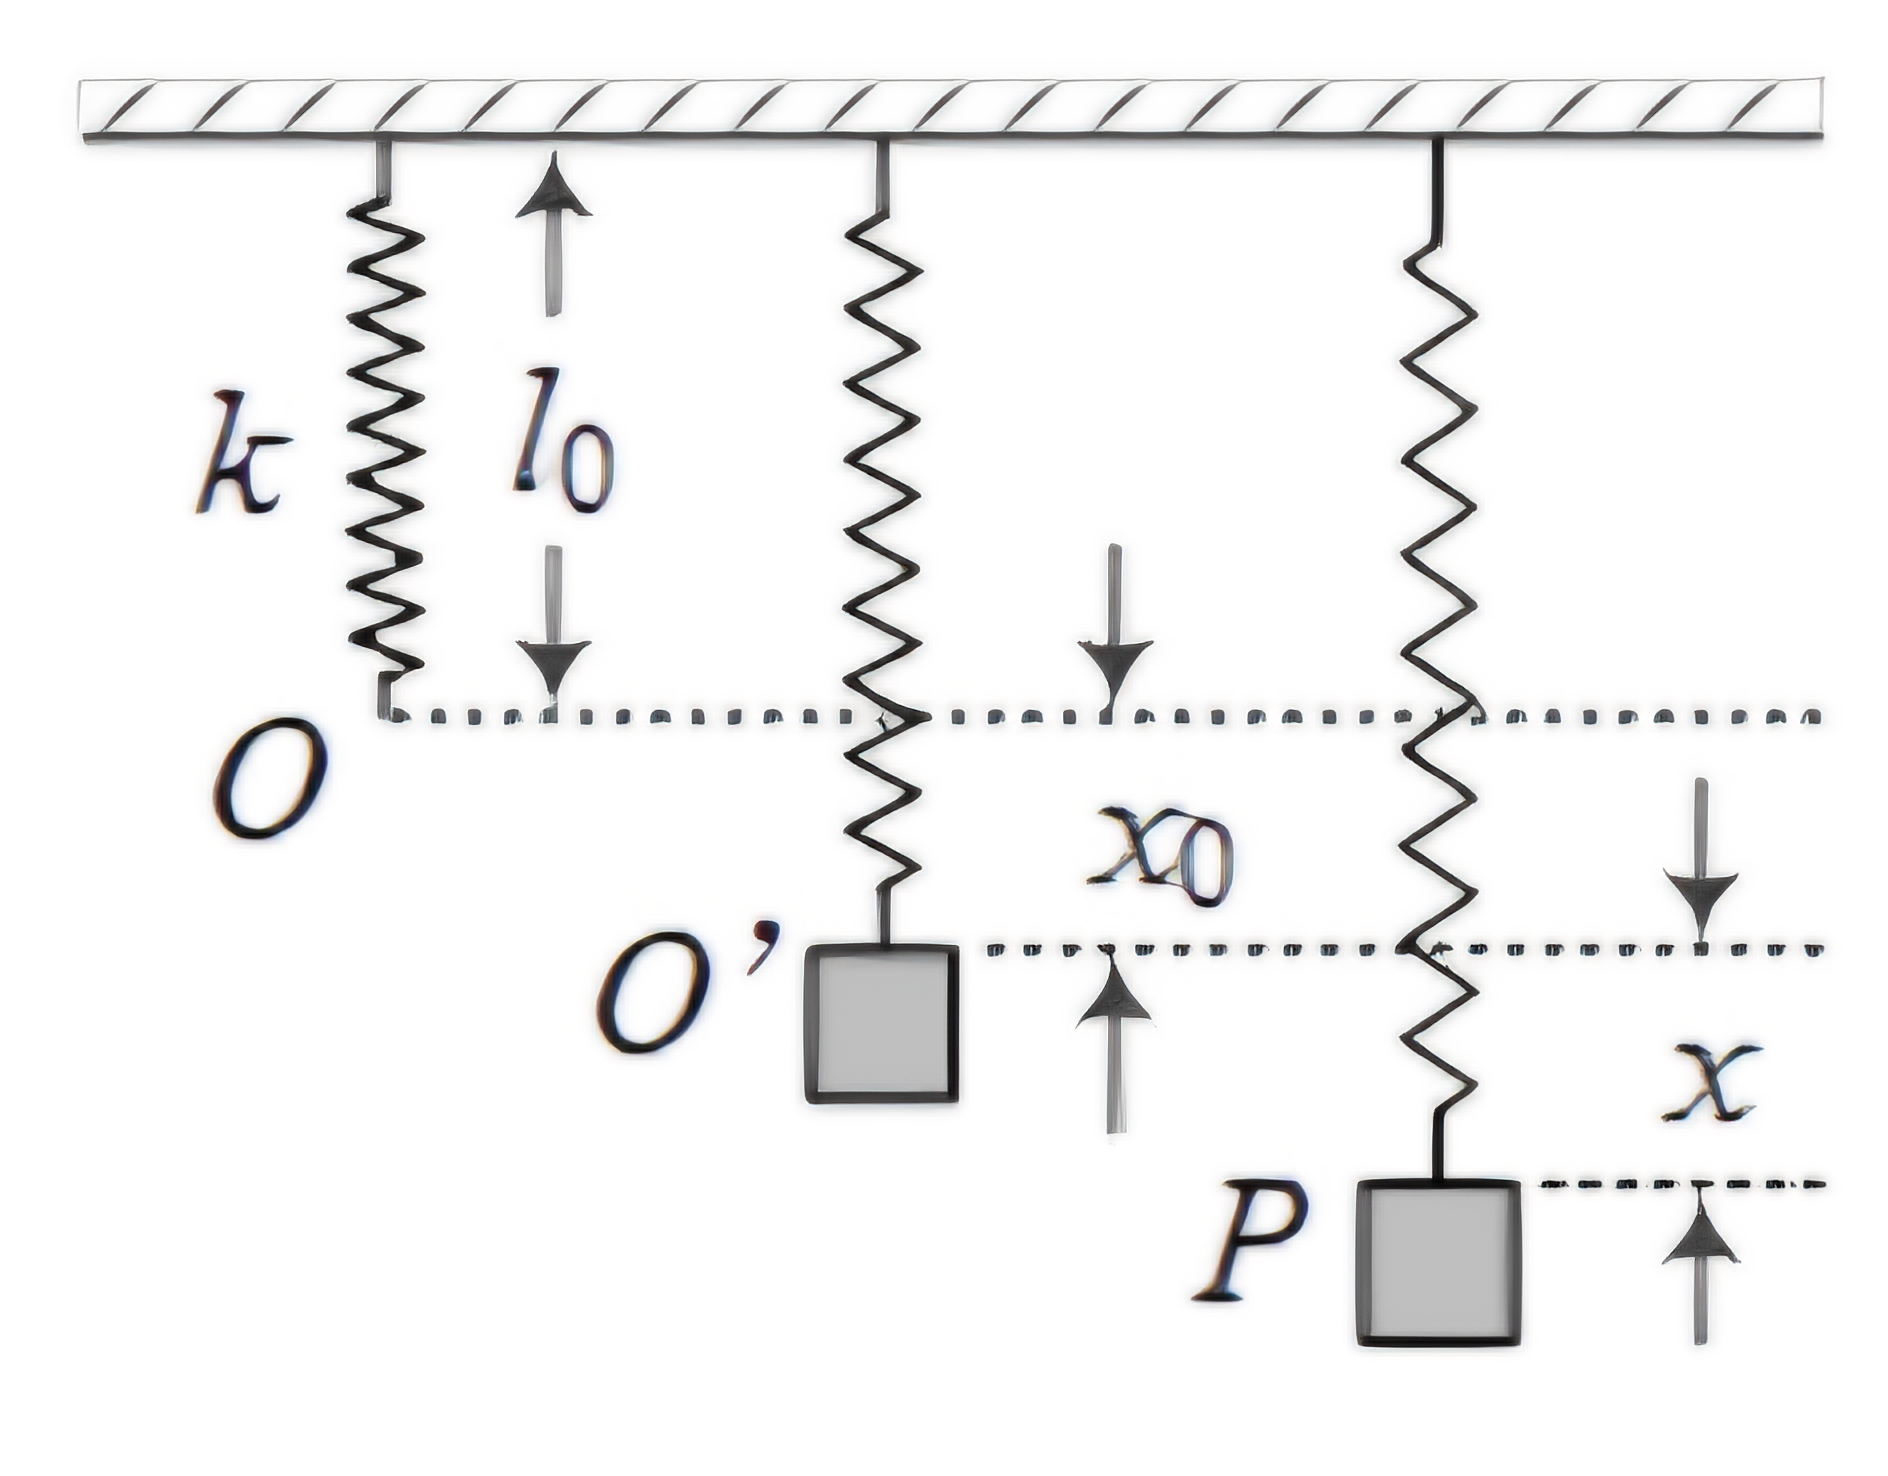
\includegraphics[scale=0.08]{"Chapter 01 images/pic2.png"}
        % \caption{}
        \label{pic2}
    \end{wrapfigure}

    \begin{align}
        \overrightarrow{r}\left(t\right) = 
        x\overrightarrow{i}\left(t\right) + y\overrightarrow{j}\left(t\right)
        + z\overrightarrow{k}\left(t\right)
    \end{align}

    分量式

    \[
    \begin{cases}
    x = x\left(t\right), \\
    y = y\left(t\right), \\ 
    z = z\left(t\right).
    \end{cases}
    \]

    从上式中消去参数得质点的{\heiti 轨迹方程}。

\subsection{位移、路程}

\subsubsection{位移\(\Delta \overrightarrow{r}\)(位置矢量的改变量)}


    \begin{wrapfigure}{r}{4cm}
        \centering
        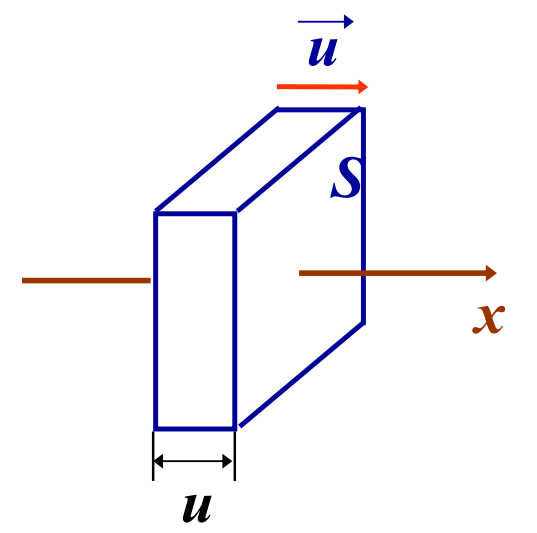
\includegraphics[scale=0.08]{"Chapter 01 images/pic3.png"}
        % \caption{}
        \label{pic3}
    \end{wrapfigure}

    \begin{align*}
        \overrightarrow{r_{A}} &=
        x_{A}\overrightarrow{i} + y_{A}\overrightarrow{j} + z_{A}\overrightarrow{k}
        ,\; \left(t_{A}\text{时}\right) \\
        \overrightarrow{r_{B}} &=
        x_{B}\overrightarrow{i} + y_{B}\overrightarrow{j} + z_{B}\overrightarrow{k}
        ,\; \left(t_{B}\text{时}\right)
    \end{align*}

    于是其位移

    \begin{align}
        \Delta \overrightarrow{r} = \overrightarrow{r_{B}} - \overrightarrow{r_{A}}
        = \left(x_{B} - x_{A}\right)\overrightarrow{i} + \left(y_{B} - y_{A}\right)\overrightarrow{j}
        + \left(z_{B} - z_{A}\right)\overrightarrow{k}
    \end{align}
    
    方向由\(A\)指向\(B\)。

\subsubsection{路程\(\Delta s\)实际轨迹}

    \begin{wrapfigure}{r}{4cm}
        \centering
        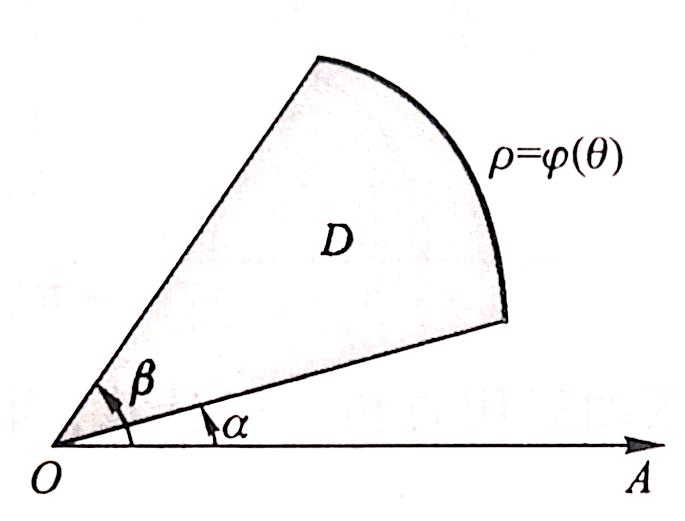
\includegraphics[scale=0.05]{"Chapter 01 images/pic4.png"}
        % \caption{}
        \label{pic4}
    \end{wrapfigure}

    从\(P_{1}\)到\(P_{2}\),路程记为\(\Delta s = \hat{P_{1}P_{2}}\)。

    位移与路程的区别:

    \begin{enumerate}
        \item 位移是适量,路程是标量;
        \item 两点之间位移是唯一的,路程不是唯一的;
        \item 一般情况下,\(\left|\Delta \overrightarrow{r}\right| \neq \Delta s\)
            \\
            在方向不变的圆周运动中,\(\left|\Delta \overrightarrow{r}\right| = \Delta s\)
            当\(\Delta t \rightarrow 0\)时,\(\left| \rmd \overrightarrow{r}\right| = \rmd s\)
            (元位移\(\rmd \overrightarrow{r} = \rmd x \overrightarrow{i} +
            \rmd y \overrightarrow{j} + \rmd z \overrightarrow{k}\))。
    \end{enumerate}

\subsection{速度}

\subsubsection{平均速度}

    \begin{wrapfigure}{r}{4cm}
        \centering
        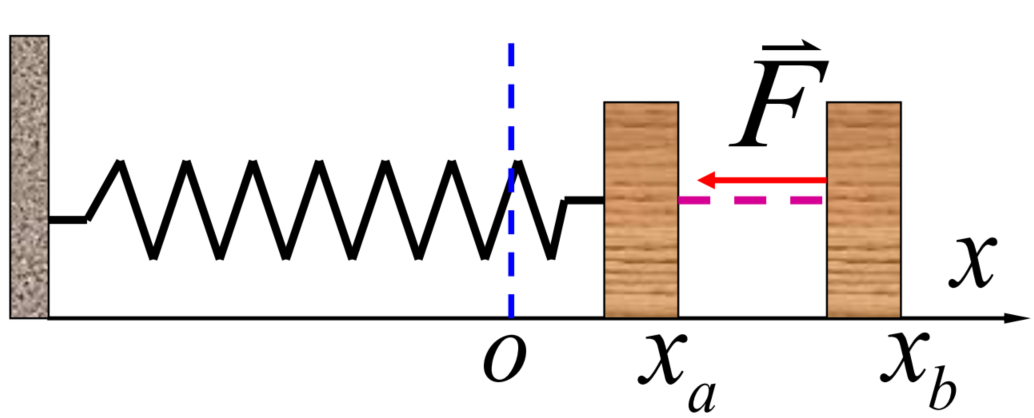
\includegraphics[scale=0.08]{"Chapter 01 images/pic5.png"}
        % \caption{}
        \label{pic5}
    \end{wrapfigure}

    在\(\Delta t\)内,质点位移(二维)为

    \begin{align*}
        \Delta \overrightarrow{r} &= \overrightarrow{r} \left(t + \Delta t\right) -
        \overrightarrow{r} \left(t\right)
        \\
        &= \Delta x \overrightarrow{i} + \Delta y \overrightarrow{j}
    \end{align*}

    \textbf{定义}
    \begin{align}
        \overrightarrow{v} = \frac{\Delta \overrightarrow{r}}{\Delta t} =
        \frac{\Delta x}{\Delta t} \overrightarrow{i} + \frac{\Delta y}{\Delta y} \overrightarrow{j}
    \end{align}

\subsubsection{瞬时速度}

    当\(\Delta t \rightarrow 0\)时,

    \begin{equation}
        \begin{aligned}
            \overrightarrow{v} = \lim_{\Delta t \rightarrow 0}\frac{\Delta \overrightarrow{r}}{\Delta t}
            &= \frac{\rmd \overrightarrow{r}}{\rmd t}
            \\
            &= \frac{\rmd x}{\rmd t} \overrightarrow{i} + \frac{\rmd y}{\rmd t} \overrightarrow{j}
            + \frac{\rmd z}{\rmd t} \overrightarrow{k}
            \\
            & = v_{x} \overrightarrow{i} + v_{y} \overrightarrow{j} + v_{z} \overrightarrow{k}
        \end{aligned}
    \end{equation}

    即有,

    \[
        v_{x} = \frac{\rmd x}{\rmd t},\; v_{y} = \frac{\rmd y}{\rmd t},\; v_{z} = \frac{\rmd z}{\rmd t}
    \]

    所以

    \begin{align}
        \left|\overrightarrow{v} \right| = \sqrt{\left(\frac{\rmd y}{\rmd t}\right)^2 +
        \left(\frac{\rmd y}{\rmd t}\right)^2 + \left(\frac{\rmd z}{\rmd t}\right)^2}
    \end{align}

    方向角

    \[
        \cos \alpha = \frac{v_x}{v},\; \cos \beta = \frac{v_y}{v}, \;\cos \gamma = \frac{v_z}{v}
    \]

    习惯上,二维情况下,用\(\tan \theta = \frac{v_y}{v_x}\)表示方向。

    同理,速率\(v = \frac{\rmd s}{\rmd t}\),而因为\(t \rightarrow 0\)时,
    有\(\left|\overrightarrow{r}\right| = s\),则

    \[
        v = \left|\overrightarrow{v}\right| =
        \left|\frac{\rmd \overrightarrow{r}}{\rmd t}\right|
        = \frac{\left|\rmd \overrightarrow{r}\right|}{\rmd t}
        = \frac{\rmd s}{\rmd t}
    \]

    即有,速度的大小等于速率。

\subsubsection{速度在自然坐标系下的表示}

    \begin{align}
        \overrightarrow{v} = \frac{\rmd s}{\rmd t}\overrightarrow{e_{t}}
        = v \overrightarrow{e_{t}}
    \end{align}

    其中,\(\overrightarrow{e_{t}} = 1\),表示方向,\(v\)表示速度大小。

\subsection{加速度}

    反应速度大小和方向随时间变化快慢。

\subsubsection{平均加速度}

    \begin{wrapfigure}{r}{4cm}
        \centering
        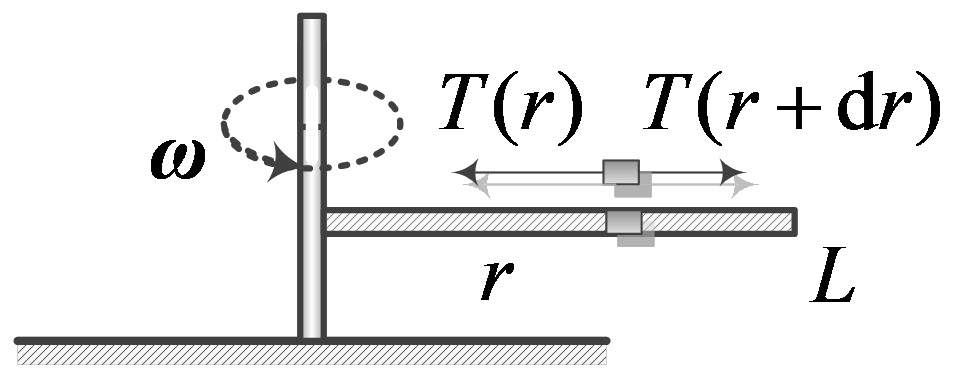
\includegraphics[scale=0.08]{"Chapter 01 images/pic6.png"}
        % \caption{}
        \label{pic6}
    \end{wrapfigure}


    \begin{align}
        \overline{\overrightarrow{a}} = \frac{\Delta \overrightarrow{v}}{\Delta t}
    \end{align}

    \(\overrightarrow{a}\)与\(\Delta \overrightarrow{v}\)的方向相同。

\subsubsection{瞬时加速度}

    特点:

    \begin{enumerate}
        \item {\color{Thistle}"矢量性"}
        \item {\color{Thistle}"瞬时性"}
        \item {\color{Thistle}"相对性"}(相对于某一参考系)
    \end{enumerate}

    \begin{equation}
        \begin{aligned}
            \overrightarrow{a} &= \lim_{\Delta t \rightarrow 0} \frac{\Delta \overrightarrow{v}}{\Delta t}
            = \frac{\rmd \overrightarrow{v}}{\rmd t} =
            \frac{\rmd^2 \overrightarrow{r}}{\rmd t^2}
            \\
            &= \frac{\rmd v_{x}}{\rmd t} \overrightarrow{i} +
            \frac{\rmd v_{y}}{\rmd t} \overrightarrow{j} +
            \frac{\rmd v_{z}}{\rmd t} \overrightarrow{k}
            \\
            &= a_{x}\overrightarrow{i} + a_{y}\overrightarrow{j}
            + a_{z}\overrightarrow{k}
        \end{aligned}
    \end{equation}

    方向角\(\alpha\)、\(\beta\)和\(\gamma\)满足

    \[
        \cos \alpha = \frac{a_x}{a},\; \cos \beta = \frac{a_y}{a}, \;\cos \gamma = \frac{a_z}{a}
    \]

    习惯上,二维时方向表示为\(\tan \theta = \frac{a_y}{a_x}\)。
    
    \begin{wrapfigure}{r}{4cm}
        \centering
        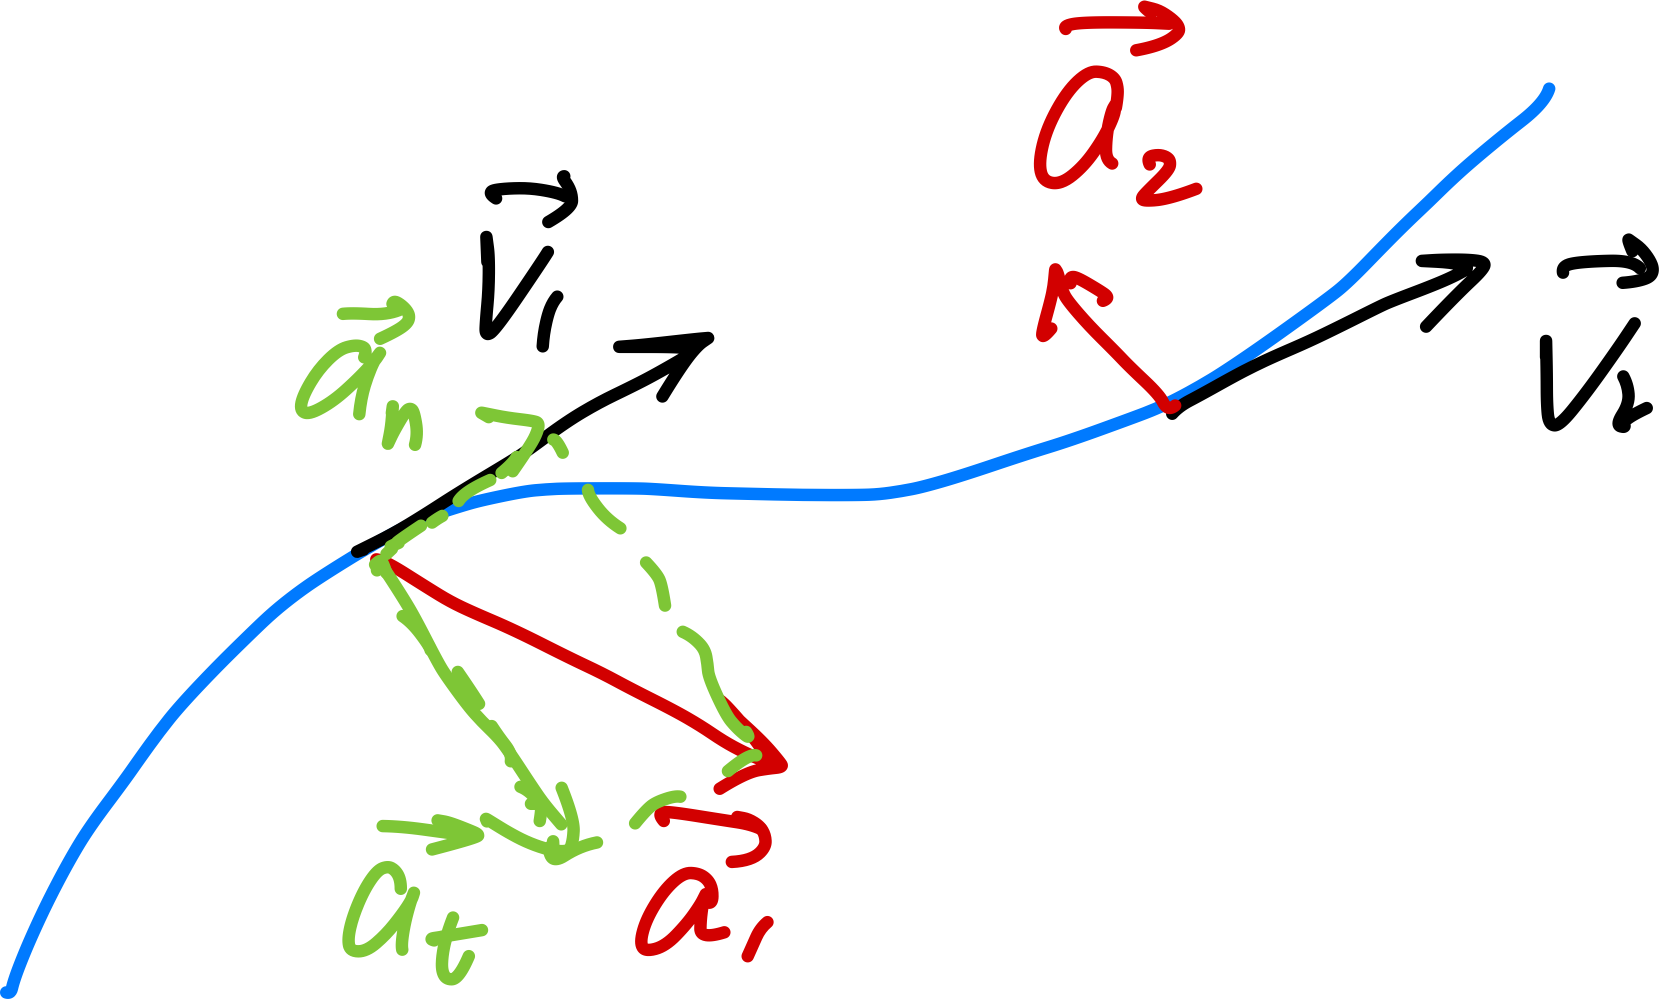
\includegraphics[scale=0.05]{"Chapter 01 images/pic7.png"}
        % \caption{}
        \label{pic7}
    \end{wrapfigure}

    加速度的方向:

    \begin{itemize}
        \item 直线运动:\(\overrightarrow{a} \parallel \overrightarrow{v}\)。
        \item 曲线运动:指向轨迹凹测。
            自然坐标系下,\(\overrightarrow{a} = \overrightarrow{a_{n}} + \overrightarrow{a_{t}}\)。
    \end{itemize}

    在变速曲线运动中,加速度的方向总是指向轨迹凹的一侧。与\(\overrightarrow{v}\)呈锐角时,运动变快;
    与\(\overrightarrow{v}\)呈钝角时,运动变快。(因为\(\Delta \overrightarrow{v}\)必定指向曲线凹的一侧。)

\section{质点运动}

\subsection{一般曲线运动与圆周运动的定义}

\subsubsection{一般曲线运动}

    特点:曲率半径随时间变化,不是定值。描述曲线运动一般选自然坐标系。

\subsubsection{圆周运动}

    圆周运动是一种常见的、简单而基本的曲线运动,是研究一般曲线运动的基础

\subsection{圆周运动}

\subsubsection{位置量的描述}

    \[
        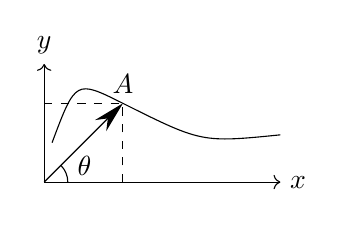
\begin{tikzpicture}
            \coordinate[label=right:$x$] (x) at (3,0);
            \coordinate[label=right:$\theta$] (theta) at (0.3,0.2);
            \coordinate[label=above:$y$] (y) at (0,1.5);
            \draw[->] (0,0) -- (x);
            \draw[->] (0,0) -- (y);
            \draw (0.1,0.5) .. controls (0.4,1.3) .. (1,1);
            \draw (1,1) .. controls (2,0.5) .. (3,0.6);
            \draw[\arrow] (0,0) -- (1,1);
            \coordinate[label=above:$A$] (A) at (1,1);
            \draw[dashed] (0,1) -- (A);
            \draw[dashed] (1,0) -- (A);
            \draw (0.3,0) arc (0:45:0.3);
        \end{tikzpicture}
    \]

    \[
        \left\{\begin{array}{l}x=r \cos \theta \\ y=r \sin \theta\end{array}\right.
    \]

    于是

    \[
        \overrightarrow{r} = x \overrightarrow{i} + y \overrightarrow{j} =
        r \cos \theta \overrightarrow{i}+ r \sin \theta \overrightarrow{j}
    \]

\subsubsection{圆周运动的角量}

    \[
        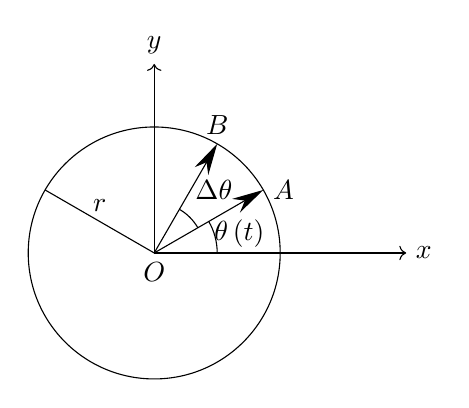
\begin{tikzpicture}[scale=0.8]
            \coordinate[label=right:$x$] (x) at (4,0);
            \coordinate[label=above:$y$] (y) at (0,3);
            \coordinate[label=below:$O$] (O) at (0,0);
            \coordinate[label=right:$A$] (A) at (1.732,1);
            \coordinate[label=above:$B$] (B) at (1,1.732);
            \coordinate[label=above:$r$] (r) at (-0.5*1.732,0.5);
            \coordinate[label={right:$\theta\left(t\right)$}] (theta) at (0.8,0.3);
            \coordinate[label=right:$\Delta \theta$] (Delta_theta) at (0.5,1);
            \draw[->] (O) -- (x);
            \draw[->] (O) -- (y);
            \draw (O) -- (-1.732,1);
            \draw[\arrow] (O) -- (A);
            \draw[\arrow] (O) -- (B);
            \draw (O) circle (2);
            \draw (1,0) arc (0:30:1);
            \draw (0.4*1.732,0.4) arc (30:60:0.8);
        \end{tikzpicture}
    \]

    角坐标\(\theta\left(t\right)\),角位移\(\Delta \theta = \theta\left(t\right) -
    \theta\left(t_0\right)\)。

    平均角速度
    
    \begin{align}
        \overline{\omega} = \frac{\Delta \theta}{\Delta t}
    \end{align}
    
    角速度
    
    \begin{align}
        \omega = \lim_{\Delta t \rightarrow 0} \frac{\Delta \theta}{\Delta t}
        = \deriv{\theta}{t}
    \end{align}

    \(\omega\)是\textbf{赝矢量},方向与\(\rmd \theta\)一致,由右手螺旋定则确定,
    且总是垂直于圆平面,沿着圆周的轴线方向。

    平均角加速度
    
    \begin{align}
        \overline{\alpha} = \frac{\Delta \omega}{\Delta t}
    \end{align}
    
    角加速度
    
    \begin{align}
        \alpha = \lim_{\Delta t \rightarrow 0} \frac{\Delta \omega}{\Delta t}
        = \deriv{\omega}{t} = \frac{\rmd^2 \theta}{\rmd t^2}
    \end{align}

\subsubsection{角量与线量的关系}

    路程与角距离的关系

    \begin{align}
        \Delta s = r \Delta \theta
    \end{align}

    速率与角速度的关系

    \begin{align*}
        b = \lim_{\Delta t \rightarrow 0} \frac{\Delta s}{\Delta t}
        = r \lim_{\Delta t \rightarrow 0} \frac{\Delta \theta}{\Delta t}
    \end{align*}

    故

    \begin{align}
        v \left(t\right) = r \omega \left(t\right)
    \end{align}

    速度

    \begin{equation}
        \begin{aligned}
            \overrightarrow{v} &= \deriv{s}{t} \overrightarrow{e_t} \\
            &= v \overrightarrow{e_t} \\
            &= r \omega \overrightarrow{e_t}
        \end{aligned}
    \end{equation}

\subsubsection{圆周运动的切向加速度和法向加速度}

    \[
        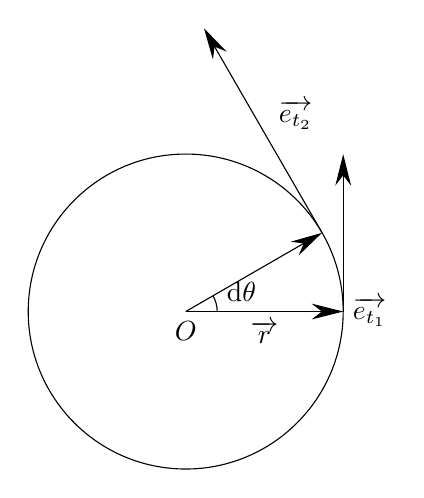
\begin{tikzpicture}
            \coordinate[label=below:$O$] (O) at (0,0);
            \coordinate[label=right:$\rmd \theta$] (dtheta) at (0.4,0.25);
            \coordinate[label=below:$\overrightarrow{r}$] (r) at (1,0);
            \coordinate[label=right:$\overrightarrow{e_{t_1}}$] (e_t_1) at (2,0);
            \coordinate[label=left:$\overrightarrow{e_{t_2}}$] (e_t_2) at (1.732,2.5);
            \draw (O) circle (2);
            \draw[\arrow] (O) -- (e_t_1);
            \draw[\arrow] (O) -- (1.732,1);
            \draw[\arrow] (e_t_1) -- (2,2);
            \draw[\arrow] (1.732,1) -- (1.732-1.5,1+1.5*1.732);
            \draw (0.4,0) arc (0:30:0.4);
        \end{tikzpicture}
    \]

    质点做变速圆周运动时

    \begin{equation}
        \overrightarrow{\alpha}=\deriv{\overrightarrow{v}}{t}=
        \frac{\rmd}{\rmd t}\left(v \overrightarrow{e}_t\right)=\deriv{\overrightarrow{v}}{t}
        \overrightarrow{e}_t+\overrightarrow{v} \deriv{\overrightarrow{e}_t}{t}
    \end{equation}

    \begin{equation}
        \alpha_{t} = \deriv{v}{t} = r \deriv{\omega}{t} = r \alpha
    \end{equation}

    因为\(\left|e_{t_1}\right| = \left|e_{t_2}\right| =1\),所以\(\left|\rmd \overrightarrow{e}\right|
    = \left|\overrightarrow{e_{t_1}}\right| \cdot \rmd \theta = \rmd \theta\)。

    当\(\rmd \theta \rightarrow 0\)时,\(\rmd \overrightarrow{e_{t}} \perp \overrightarrow{e_{t_1}}\),
    故\(\rmd \overrightarrow{e_{t}}\)的方向与\(\overrightarrow{e_{n}}\)方向相同,即

    \begin{align}
        \rmd \overrightarrow{e_{t}} = \rmd \theta \overrightarrow{e_n}
    \end{align}

    所以

    \[
        v \deriv{\overrightarrow{e_t}}{t} = v \deriv{\theta}{t} \overrightarrow{e_{n}} = v \omega
    \]

    于是

    \begin{align}
        \alpha_n &= \omega v \\
        &= \frac{v^2}{r}
    \end{align}

    综上所述,切向加速度\(\overrightarrow{\alpha_t} = \deriv{v}{t} \overrightarrow{e_t}, \;
    \alpha_t = \deriv{v}{t}\);法向加速度\(\overrightarrow{\alpha_t} = \frac{v^2}{r} \overrightarrow{e_n},
    \; \alpha_n = \frac{v^2}{r} = \omega^2r = \omega v\)。

\subsection{一般曲线运动}

    同圆周运动理知,

    \begin{align}
        \alpha_t = \deriv{v}{t}
    \end{align}

    \begin{align}
        \alpha_n = \frac{v^2}{\rho}\; \text{(\(\rho\)是曲率半径)}
    \end{align}

    而\(\overrightarrow{\alpha} = \overrightarrow{\alpha_t} + \overrightarrow{\alpha_n}\),所以

    \begin{align}
        \left|\overrightarrow{\alpha}\right| = \sqrt{\alpha_t^2 + \alpha_n^2}
    \end{align}

    自然坐标系下的加速度表达式:
    
    \begin{align}
        \overrightarrow{\alpha_t} = \deriv{v}{t} \overrightarrow{e_t} =
        \frac{\rmd^2 s}{\rmd t^2} \overrightarrow{e_t}
    \end{align}

    \begin{align}
        \overrightarrow{\alpha_n} = \frac{v^2}{\rho} \overrightarrow{e_n}
    \end{align}

\section{相对运动}

\subsection{时间与空间}

    在两个相对作直线运动的参考系中,时间的测量是绝对的,空间的测量也是绝对的,与参考系无关。

    时间和长度的的绝对性是经典力学或牛顿力学的基础。

    在两个相对作直线运动的参考系中, 时间的测量是绝对的,空间的测量也是绝对的, 与参考系无关, 时间和长度的的绝对性是经典力学或牛顿力学的基础。

\subsection{相对运动公式}

    \begin{wrapfigure}{r}{4cm}
        \centering
        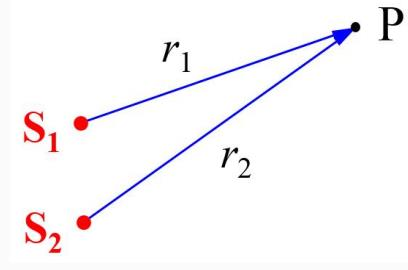
\includegraphics[scale=0.3]{"Chapter 01 images/pic8.png"}
        % \caption{}
        \label{pic8}
    \end{wrapfigure}

    如右图,\(\overrightarrow{r_{OP}} = \overrightarrow{r_{OO^{'}}} + \overrightarrow{r_{O^{'}P}}\),

    对方程两边对时间求导数,得

    \begin{align*}
        \deriv{\overrightarrow{r_{OP}}}{t} = \deriv{\overrightarrow{r_{OO^{'}}}}{t} +
        \deriv{\overrightarrow{r_{O^{'}P}}}{t}
    \end{align*}

    即

    \begin{align}
        \overrightarrow{v_{P \rightarrow O}} = \overrightarrow{v_{P \rightarrow O^{'}}} +
        \overrightarrow{v_{O^{'} \rightarrow O}}
    \end{align}

    (绝对速度 = 相对速度 + 牵连速度)

    方程两边对时间求导数,得

    \begin{align}
        \overrightarrow{a_{P \rightarrow O}} = \overrightarrow{a_{P \rightarrow O^{'}}} +
        \overrightarrow{a_{O^{'} \rightarrow O}}
    \end{align}

    (绝对加速度 = 相对加速度 + 牵连加速度)

    如果\(\overrightarrow{u}\)是恒矢量,则\(\deriv{\overrightarrow{u}}{t} = 0\),
    \(\overrightarrow{a_{PO}} = \overrightarrow{a_{PO^{'}}}\),\(\overrightarrow{a_{O^{'}O}} = 0\)。

    注意:

    \begin{enumerate}
        \item 当\(\overrightarrow{u}\)接近光速时,速度变换、加速度变换不成立;
        \item 仅仅讨论\(\overrightarrow{u} = u_x \overrightarrow{i}\)的情况(\(u_x\)为常数),
        即水平方向有变换,其他方向上没有变换。
    \end{enumerate}

\subsection{伽利略速度变换}

    \begin{wrapfigure}{r}{4cm}
        \centering
        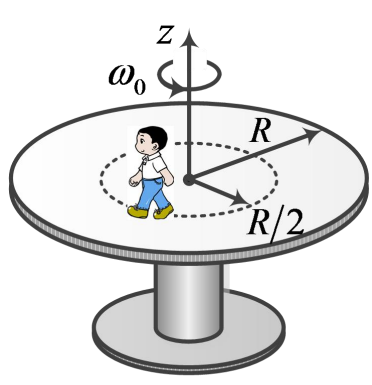
\includegraphics[scale=0.4]{"Chapter 01 images/pic9.png"}
        % \caption{}
        \label{pic9}
    \end{wrapfigure}

    \begin{align}
        \overrightarrow{v} = \overrightarrow{v}^{'} + \overrightarrow{u}
    \end{align}

    绝对速度\(\overrightarrow{v} = \deriv{\overrightarrow{r}}{t}\),相对速度\(\overrightarrow{v}^{'} =
    \deriv{\overrightarrow{r}^{'}}{t}\),牵连速度\(\overrightarrow{u}\)。

    加速度关系:

    \begin{align}
        \deriv{\overrightarrow{v}}{t} = \deriv{\overrightarrow{v}^{'}}{t} + \deriv{\overrightarrow{u}}{t}
    \end{align}

    若\(\deriv{\overrightarrow{u}}{t} = 0\),则\(\overrightarrow{a} = \overrightarrow{a}^{'}\)

\section{例题}

\subsection{Problem 1}

    在离水面高为\(h\)的岸上,有人用绳拉船靠岸,如图所示。设人以匀速率\(v_{0}\)收绳,试求:
    当船距岸边\(x_{0}\)时,船的速度和加速度的大小各是多少?

    \[
        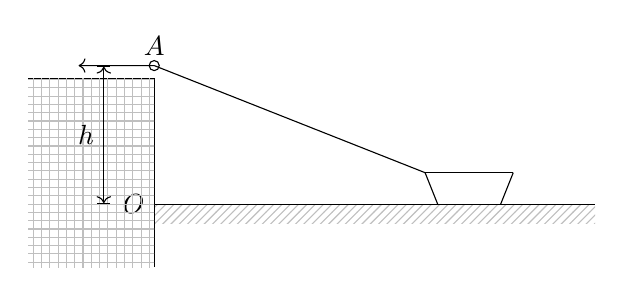
\begin{tikzpicture}[scale=0.8]
            \coordinate[label=left:$O$] (O) at (0,0);
            \coordinate[label=above:$A$] (A) at (0,2.2);
            \fill[pattern=north east lines, pattern color=gray!50] (0,0) rectangle (7,-0.3);
            \draw (0,-1) -- (0,2);
            \draw (O) -- (7,0);
            \draw (0,2) -- (-2,2);
            \fill[pattern=grid, pattern color=gray!50] (0,-1) rectangle (-2,2);
            \draw (A) circle (0.08);
            % 小船
            \draw (4.5,0) -- (5.5,0);
            \draw (4.5,0) -- (4.3,0.5);
            \draw (5.5,0) -- (5.7,0.5);
            \draw (4.3,0.5) -- (5.7,0.5);
            % 绳子
            \draw (A) -- (4.3,0.5);
            \draw[->] (A) -- (-1.2,2.2);
            % 尺寸标注
            \draw[|<->|] (-0.8,0) -- (-0.8,2.2) node[midway, left] {$h$};
        \end{tikzpicture}
    \]
    \\

    \textbf{Solution}
    \\

    \textbf{Part One}

    建立如图所示的坐标系。

    \[
        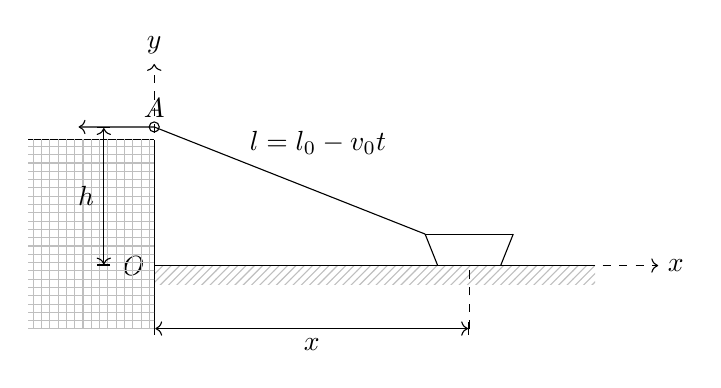
\begin{tikzpicture}[scale=0.8]
            \coordinate[label=left:$O$] (O) at (0,0);
            \coordinate[label=above:$A$] (A) at (0,2.2);
            \fill[pattern=north east lines, pattern color=gray!50] (0,0) rectangle (7,-0.3);
            \draw (0,-1) -- (0,2);
            \draw (O) -- (7,0);
            \draw (0,2) -- (-2,2);
            \fill[pattern=grid, pattern color=gray!50] (0,-1) rectangle (-2,2);
            \draw (A) circle (0.08);
            % 小船
            \draw (4.5,0) -- (5.5,0);
            \draw (4.5,0) -- (4.3,0.5);
            \draw (5.5,0) -- (5.7,0.5);
            \draw (4.3,0.5) -- (5.7,0.5);
            % 绳子
            \draw (A) -- (4.3,0.5);
            \draw[->] (A) -- (-1.2,2.2);
            \coordinate[label={above:$ l = l_{0} - v_{0}t $}] (rope) at (2.6,1.6);
            % 尺寸标注
            \draw[|<->|] (-0.8,0) -- (-0.8,2.2) node[midway, left] {$h$};
            \draw[|<->|] (0,-1) -- (5,-1) node[midway, below] {$x$};
            \draw[dashed] (5,-1) -- (5,0);
            % 坐标系
            \coordinate[label=right:$x$] (x) at (8,0);
            \coordinate[label=above:$y$] (y) at (0,3.2);
            \draw[->,dashed] (O) -- (x);
            \draw[->,dashed] (O) -- (y);
        \end{tikzpicture}
    \]

    设初始时刻,船与岸上\(A\)点之间的绳长为\(l_{0}\)。在任意时刻船离岸边的距离为\(x\),
    绳长为\(l_{0}\)。船在运动过程中,\(l\)和\(x\)均是时间\(t\)的函数。

    由题意,\(l = l_{0} - v_{0}t\),所以

    \[
        v_{0} = - \deriv{l}{t}
    \]

    又由几何关系

    \[
        l^{2} = x^{2} + h^{2}
    \]

    对上式两边同时对\(t\)求导,可得

    \[
        2 l \deriv{l}{t} = 2x \deriv{x}{t}
    \]

    则船的运动速度为

    \[
        v = \deriv{x}{t} = \frac{l}{x} \deriv{l}{t} = -\frac{l}{x} v_{0}
    \]
    \\

    \textbf{Part Two}

    再将速度对时间\(t\)求导,即可得到船的加速度为

    \[
        a = \deriv{v}{t} = - \frac{v_{0}}{x^{2}} \left(x \deriv{l}{t} - l \deriv{x}{t}\right)
        = -\frac{v_{0}^{2} h^{2}}{x^{3}}
    \]
    \\

    \textbf{Part Three}

    令\(x=x_{0}\),得船在离岸边为\(x_{0}\)时的速度和加速度分别为

    \[
        v = \frac{\sqrt{x_{0}^{2} + h^2}}{x_{0}} v_{0},\;
        a = -\frac{v_{0}^{2} h^{2}}{x_{0}^{3}}
    \]
\end{document}
